\PassOptionsToPackage{sols}{handout}
\documentclass[main]{subfiles}
\setcounterrefbeforedot{chapter}{m-ws2-5}
\setcounterrefafterdot{section}{m-ws2-5}
\addtocounter{section}{-1}
\usepackage{solutions}

\begin{document}

\ifSubfilesClassLoaded{%
  \chaptermark{\chaptertwo}
}{}

\section{Modeling Periodic Phenomena} \label{ws2-5}

\begin{enumerate}
\item 
  \note{This is to clarify the meaning of ``periodic''.  I'll start with
    an informal definition like ``the graph repeats,'' which is pretty
    ambiguous, and then I'll ask what they think of each of these.  I hope
    that, by discussing these as a class, everyone will get a clear
    understanding of what periodic means. }

  Recall that a \emph{periodic} function is a function whose values eventually repeat. More precisely, a periodic function shows identical behavior over successive intervals of length $T$, where $T$ is known as the period.

  Circular motion is periodic, but there are many other phenomena that behave periodically. Which of the following phenomena would you describe as periodic?  Which are not periodic?

  \begin{enumerate}
  \item
    \begin{problem}
      A normal EKG:
      \begin{minipage}{3in}
        
\includegraphics[width=2.5in]{images/ekg-crop2}
      \end{minipage}
    \end{problem}
    \pspace{0.25in}

    \begin{solution}
      While not perfectly periodic, it seems reasonable to model this
      function using a periodic function; the piece highlighted in red
      below appears to repeat over and over:
      \begin{center}
        
\includegraphics[width=3in]{images/ekg-crop2-highlighted}
      \end{center}
    \end{solution}

  \item
    \begin{problem}
      Torsades de pointes is a rare arrythmia of the heart which can lead
      to sudden death if untreated.

      \begin{tabular}{c c}
        
\includegraphics[width=2.5in]{images/torsades3} &         
        
\includegraphics[width=2.5in]{images/torsades-model} \\
        Actual EKG % http://www.themdsite.com/physicians.cfm
        & Model of
        Torsades de pointes
      \end{tabular}
    \end{problem}
    \pspace{0.5in}

    \begin{solution}
      The model of Torsades de pointes shown on the right is periodic; the
      red piece is repeated over and over:
      \begin{center}
        
\includegraphics[height=0.4in]{images/torsades-model-highlighted}
      \end{center}
    \end{solution}    

  \item
    \begin{problem}
      At the Mauna Loa observatory in Hawaii, the amount of carbon dioxide
      in the atmosphere has been measured every month since 1958.  A graph of the data is
      shown below.
    \end{problem}

    
\includegraphics[width=2.4in]{images/mauna-loa}


    \begin{solution}
      This function is not periodic; rather than repeating, the graph has
      a general trend of increasing. 
    \end{solution}    

  \item
    \begin{problem}
      In Fall River, MA, the water level is measured every 6 minutes.
      A graph of the data from January 1, 2012 to January 6, 2012 is
      shown below.
    \end{problem}

    
\includegraphics[width=2.4in]{images/fall-river-tides}


    \begin{solution}
      It seems very reasonable to model this function using a periodic
      function; the piece highlighted in red
      below appears to repeat over and over:
      \begin{center}
        
\includegraphics[width=2.4in]{images/fall-river-tides-highlighted}
      \end{center}
    \end{solution}

  \end{enumerate}

\item 
\begin{problem}
    One of the contexts from the previous problem can be reasonably modeled using a sinusoidal function. Which one? Why would a sinusoid not be a good choice for modeling the others?
\end{problem}
\pspace{\vfill}

\begin{solution}
    The final example, the water level in Fall River, MA, can be reasonably modeled using a sinusoidal function. The water level has the key characteristics of a sinusoid: it is roughly periodic, has regular peaks and values (which indicates the existence of a period), which are centered about a midline.
\end{solution}

\end{enumerate}
\pspace{\newpage}

\begin{enumerate}[resume]
  \item
    \begin{problem}
      The graph below shows the water level (in feet) in Fall River, MA from January 1, 2012 to January 6, 2012. Estimate the midline, amplitude, and period.
    \end{problem}

    
\includegraphics[width=2.4in]{images/fall-river-tides}
    
\begin{solution}
    The peaks and troughs of the water level reach approximately 24.5 feet and 21.5 feet, respectively. This means the amplitude is 1.5 feet, and the midline occurs at roughly $y=23$. There are two full cycles between consecutive days. Specifically, we go from trough to peak to trough to peak and back to trough. This means that it takes 12 hours or half a day to complete one full cycle, starting at a trough and returning to a trough one time.
\end{solution}
\item
\begin{problem}
    Come up with the equation of a sinusoid to model the data given in the previous problem. Make sure to define what your variables represent.
\end{problem}

\pspace{\vfill}
\begin{solution}
    Let $W$ represent water level of Fall River, MA, in feet. Let $t$ represent time in days, starting from January 1, 2012. \\
    We begin at a trough, so we will use $-\cos x$ as our parent function. The general form will follow $-A\cos(Bt)+C$. $A$ corresponds to amplitude, so it is set to 1.5. $C$ corresponds to our midline, and is set to 23.  \\
    $B$ is the constant that adjusts the period; it converts the fraction of a period that has elapsed into radians, the input we need for the cosine function. We take the number of days $t$, divide by our period 0.5, which gives the number of periods that have elapsed, and multiply by $2\pi$, which will completely convert our $t$ days into radians. This is why $B=\frac{2\pi}{\text{period}}=\frac{2\pi}{0.5}=4\pi$\\
                                         
            Our model is \fbox{$W=-1.5\cos(4\pi t)+23$}
\end{solution}                                                                                              
\item
\begin{problem}
Every time your heart beats, your blood pressure increases to a maximum (known as systolic pressure) due to the force of your heart pumping, then decreases back to a minimum (known as diastolic pressure). 

Suppose a person at rest's systolic pressure is 120 millimeters of mercury (mmHg), and their diastolic pressure is 80 mmHg. Their resting heart rate is 60 beats per minute.
\end{problem}

\begin{enumerate}
\item 
\begin{problem}
Given that the person's blood pressure is currently at a minimum ($t=0$), graph their blood pressure $P$ (in mmHg) as a sinusoidal function of time $t$ (in seconds.)
\end{problem}
\pspace{\stretch{2}}

\begin{solution}
     We're told that the maximum corresponds to a person's systolic pressure, which is 120 mmHg in this example. The minimum, which we're told is the diastolic pressure, is 80 mmHg. We're told we begin at a minimum. The midline is halfway between the maxima and minima, so ours will be at $y=100$. We are told their resting heart rate is 60 beats per minute and that every time the heart beats, blood pressure reaches a maximum. These two facts together indicate the period, which is 1/60 of a minute or 1 second. The latter is what we'll use because $t$ is defined to be in seconds. 
\end{solution}
\item
\begin{problem}
    Come up with a formula for the sinusoidal function you graphed.
\end{problem}
\pspace{\vfill}

\begin{solution}
     We went through a lot of the reasoning necessary to sketch our function. We're told that blood pressure is at a minimum at $t=0$, so we'll use $-\cos x$ as our parent function to start building our model, since we need to be at a trough in our sinusoid. The general form will follow $P(t)=-A\cos(Bt)+C$.\\
    Amplitude is half the difference between the maxima and the minima of the function. We're told that the maximum corresponds to a person's systolic pressure, which is 120 mmHg in this example. The minimum, which we're told is the diastolic pressure, is 80 mmHg. The difference is 40, so the amplitude is 20. The midline is halfway between the maxima and minima, so ours will be at $y=100$. We are told their resting heart rate is 60 beats per minute and that every time the heart beats, blood pressure reaches a maximum. These two facts together indicate the period, which is 1/60 of a minute or 1 second. The latter is what we'll use because $t$ is defined to be in seconds. \\
    Our pressure function is \fbox{$P(t)=-20\cos(2\pi t)+100$}
\end{solution}
\end{enumerate}

\item 
\begin{problem}
Some stars, known as \emph{variable stars}, brighten and dim periodically. The brightness of one such star is modeled by the function $f(t)=8-2\sin(\frac{\pi}{150}t)$, where $t$ is measured in days. Determine the period of the star and its maximum and minimum brightness.

\end{problem}
\pspace{\vfill}
\begin{solution}
    To determine the period, we investigate the coefficient on $t$ within the sine function. The coefficient $\frac{\pi}{150}$ acts a factor that converts from $t$'s time units to radians, which we can then input into the sine function. This factor tells us that every 150 days is the equivalent of $\pi$ radians. We know that $2\pi$ radians is one period for the sine function; the corresponding number of days for one period is therefore \fbox{300 days}.\\
    Our midline is 8 in this model, and in order to determine maximum and minimum brightness, we notice that amplitude, which is the absolute value of the coefficient on the sine function, is 2. This means our maximum brightness will be \fbox{10 brightness units} and our minimum brightness will be \fbox{6 brightness units} (whatever those units may be!).
\end{solution}
\end{enumerate}

\pspace{\newpage}

\begin{enumerate}[resume]
\item 
    Suppose you are riding a Ferris wheel, and your height $h$ above the ground in feet at time $t$ (in seconds) is given by $h=70\sin(\frac{\pi}{20}t)+80$.
\begin{enumerate}
\item
\begin{problem}
Sketch the graph of the function and label the axes.
\end{problem}
\pspace{\stretch{2}}

\begin{solution}
    \begin{center}
        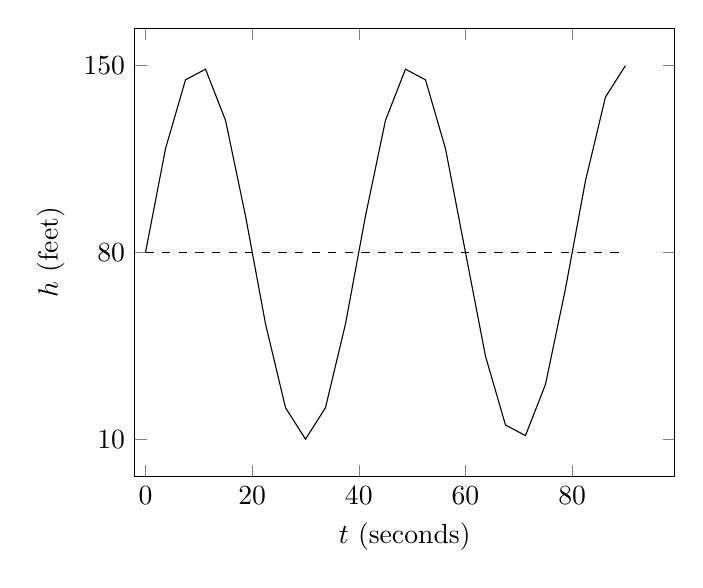
\begin{tikzpicture}
            \begin{axis}[
            xlabel=$t$ (seconds), ylabel=$h$ (feet),
            xmin=-2, ytick={10,80,150}
            ]
                \addplot[domain=0:90] {70*sin(deg(pi*x/20))+80};
                \addplot[domain=0:90, dashed] {80};
            \end{axis}
        \end{tikzpicture}
    \end{center}
\end{solution}

\item
\begin{problem}
How big is the Ferris wheel? How long does it take to complete one full revolution?
\end{problem}
\pspace{\vfill}

\begin{solution}
    The amplitude gives us how far from the midline we get while riding the Ferris wheel. In this physical example, the midline is at the horizontal middle of the wheel, and the coefficient on the sine function, which is 70), indicates we go 70 feet above and below that while riding. That means the Ferris wheel has a \fbox{70 foot radius or 140 foot diameter.}\\
    The time to complete a full revolution is the period. The coefficient on $t$ inside the sine function controls this. It acts as a conversion factor between our units of time that $t$ is counted in and radians, which the sine function takes as input. The coefficient $\frac{\pi}{10}$ indicates that 10 seconds is the equivalent of $\pi$ radians, which we know to be half a period for the sine function. This means that a full period, or the time to complete a full revolution will be \fbox{20 seconds.}
\end{solution}
% \item 
% \begin{problem}
% Find the next 4 times after $t=0$ when you are 110 feet above the ground.
% \end{problem}

\item 
\begin{problem}
    Suppose you want to adjust the equation so that $t=0$ corresponds to when you are at the bottom of the Ferris wheel. Which of the following equations would work? How do you know?
    \probonly{
    \begin{tasks}[label-width=12pt, label=\roman*., after-item-skip=72pt, after-skip=72pt](2)
    \task $h=70\sin(\frac{\pi}{20}t-10)+80$
    \task $h=70\sin(\frac{\pi}{20}t- \frac{\pi}{2})+80$
    \task $h=70\sin\!\left[\frac{\pi}{20}(t-10)\right]+80$
    \task $h=70\sin\!\left[\frac{\pi}{20}(t-\frac{\pi}{2})\right]+80$
    \end{tasks}
    }
    \solonly{
    \begin{tasks}[label-width=12pt, label=\roman*.](2)
    \task $h=70\sin(\frac{\pi}{20}t-10)+80$
    \task $h=70\sin(\frac{\pi}{20}t- \frac{\pi}{2})+80$
    \task $h=70\sin\!\left[\frac{\pi}{20}(t-10)\right]+80$
    \task $h=70\sin\!\left[\frac{\pi}{20}(t-\frac{\pi}{2})\right]+80$
    \end{tasks}
    }

\end{problem}

\begin{solution}
    We can determine this by evaluating each of these function when $t=0$. We are looking to see whether the input to the sine function corresponds to a position on the unit circle where the sine value is $-1$, which is the lowest point of the function, which would be the bottom of the wheel. Option i has us evaluating $\sin(-10)$ when $t=0$, which is not the input to sine that we're looking for to achieve the lowest point. Similarly option iv has us evaluating $\sin(\frac{-\pi^2}{40})$, which is also not a position where sine outputs its minimum. \fbox{Options ii and iii} both have us evaluating $\sin(-\frac{\pi}{2})$, which is a location on the unit circle where the sine function achieves its minimum, and so this will correspond to the rider being at the bottom of the Ferris Wheel at that time.
\end{solution}
\item 
\begin{problem}
    What's another way to write the equation so that the minimum value occurs at $t=0$?
\end{problem}
\pspace{\vfill}

\begin{solution} 
By using $-\cos x$ as the parent function, we have selected a sinusoid that begins at a trough at $t=0$. We keep amplitude, period, and balance line the same, giving us \fbox{$h=-70\cos(\frac{\pi}{20}t)+80$}

\end{solution}

\end{enumerate}


% \item 
% \begin{enumerate}
% \item
% \begin{problem}
%     Sketch the graph of $y=\cos(3t+\frac{\pi}{2})$. Which transformation should be done first? How do you know?
% \end{problem}
% \pspace{\stretch{2}}

% \item
% \begin{problem}
%     Rewrite the equation using sine instead of cosine.
% \end{problem}
% \pspace{\vfill}
% \end{enumerate}

\end{enumerate}

\pspace{\newpage}

\begin{enumerate}[resume]
\item 

\note{This problem foreshadows Lesson 11 on derivatives of trig
  functions, where students will see
  the formal statement of the Squeeze Theorem/Sandwich Theorem in the
  context of $\lim_{x\to0}\frac{\sin x}{x}$.

  If you have time to talk about this, you may want to introduce the
    term ``envelope function'': since $\sin x$ oscillates between $-1$ and
    $1$, $e^{0.05 x} \sin x$ oscillates between $-e^{0.05 x}$ and $e^{0.05
      x}$, and the two functions $\pm e^{0.05 x}$ are called ``envelopes''
    for $e^{0.05 x} \sin x$.  (As far as I can tell, there is not a
    commonly accepted definition for envelope in this context, so don't
    try to define too precisely.)  Generally, students' first step in
    understanding oscillating functions like this will be to draw the
    envelope functions.

    $\lim_{x \to \infty} e^{0.05 x} \sin x$ is a type of
    limit that they've never encountered before, so you'll need to let
    them know that it's DNE and help them adjust their mental image of
    what a limit is.
  }
Sine and cosine can be used together with other functions to model oscillating, non-periodic behavior. 

In this problem, we will investigate the function 
  $f(x)=e^{0.05x} \sin x$.

  \begin{enumerate}

    \item
      \begin{problem}
        Given that $\sin x$ oscillates between $1$ and $-1$, $e^{0.05x}\sin x$ oscillates between which two functions?
        \[
        \cfitb{1in}{-e^{0.05x}} 
        \hspace{12pt} \leq \hspace{12pt}
        e^{0.05x}\sin x
        \hspace{12pt} \leq \hspace{12pt}
        \cfitb{1in}{e^{0.05x}}
        \]
      \end{problem}

    \item

      \begin{problem}
        What happens to the two functions you wrote down
        as $x \to \infty$? What about as $x \to -\infty$?
      \end{problem}
      \pspace{\vfill}

      \begin{solution}
        As $x \to \infty$, $e^{0.05x} \to \infty$ and 
        $-e^{0.05x} \to -\infty$.
        As $x \to -\infty$, $e^{0.05x}$ and $-e^{0.05x}$ both approach
        zero.
      \end{solution}

    \item
    \begin{problem}
      What can you say about $\lim\limits_{x\to\infty} e^{0.05x}\sin x$?
      What about $\lim\limits_{x\to-\infty} e^{0.05x}\sin x$?
    \end{problem}
    \pspace{\vfill}

    \begin{solution}
        Since we know that $f(x)e^{0.05x}\sin x $ is always between
        $e^{0.05x}$ and $-e^{0.05x}$, as $x\to-\infty$, $f(x)$ gets
        ``squeezed'' closer and closer to zero. Thus, 
        \fbox{$\lim\limits_{x\to-\infty} e^{0.05x}\sin x = 0$.}

        As $x \to \infty$, $f(x)$ will be oscillating up and down
        between $e^{0.05x}$ and $-e^{0.05x}$, and so it will not
        approach any particular value. Thus, 
        \fbox{$\lim\limits_{x\to\infty} e^{0.05x}\sin x$ does not exist.}
    \end{solution}
    
  \end{enumerate}

\item Challenge: match each equation below to its corresponding graph. 
\begin{tasks}(4)
     \task $y=e^{0.05x}\cdot\sin(x)$
    \task $y=\frac{1}{5}x+\sin(x)$
      \task $y=\frac{1}{5}x \cdot \sin(x)$ 
     \task $y=e^{0.05x}+\sin(x)$
\end{tasks}

 \begin{multicols}{2}
      \begin{enumerate}[label=(\arabic*)]
      \item \raisebox{2ex-\height}{
\includegraphics[width=1.8in]{images/trig-graph-matching-1-2}} 
      \item \raisebox{2ex-\height}{
\includegraphics[width=1.8in]{images/trig-graph-matching-1-5}}
       \item \raisebox{2ex-\height}{
\includegraphics[width=1.8in]{images/trig-graph-matching-1-1}}
      \item \raisebox{2ex-\height}{
\includegraphics[width=1.8in]{images/trig-graph-matching-1-4}} 
      \end{enumerate}
      \end{multicols}
\end{enumerate}

\end{document}